\documentclass{article}
\usepackage{iclr2026_conference,times}
\input{math_commands.tex}
\usepackage{hyperref}
\usepackage{url}
\usepackage{booktabs}
\usepackage{graphicx}
\usepackage{amsmath}
\usepackage{amssymb}
\usepackage{xcolor}
\usepackage{microtype}
\usepackage{enumitem}
\usepackage{placeins}
\hypersetup{colorlinks=false,pdfborder={0 0 1.8},citebordercolor={0 1 0},linkbordercolor={0 0.85 0},urlbordercolor={0 0.55 1}}
\setlist[itemize]{leftmargin=1.2em,itemsep=0.15em,topsep=0.2em}
\raggedbottom
\title{World-Model Audits From Failed Robot Rollouts}
\author{Anonymous Authors}
\begin{document}
\maketitle
\begin{abstract}
Robot world models can fail in a way that is actionable but hidden: after a bad rollout, the planner knows that prediction was wrong but not whether the missing mechanism was friction, compliance, occlusion persistence, contact-mode change, actuator lag, payload shift, sensor dropout, or compound aliasing. We rebuild Paper 118 as a v5 expanded audit around counterfactual\_mechanism\_audit\_v5, a counterfactual mechanism-audit controller that converts failed rollouts into a mechanism posterior and then chooses repair, probe, abstention, or conservative fallback. The local CPU-only suite contains 230,400 main rollout cells, 38,400 ablation cells, 161,280 stress cells, 107,520 fixed-budget cells, and 24 failure cases. On the hard slice, v5 reaches success 0.80583 and utility 0.68463, versus 0.70615 and 0.42095 for the strongest non-oracle comparator, proposed\_failed\_rollout\_audit\_v4\_1. It improves mechanism F1 by 0.08835, reduces invalid repair by -0.04046, repeat failure by -0.03822, damage by -0.01269, probe cost by -0.03908, and budget violation by -0.05457. The terminal state is \texttt{STRONG\_REVISE}, not ICLR-main ready, because real robot or accepted high-fidelity validation is still absent.
\end{abstract}
\section{Motivation}
The literature on world models, latent dynamics, and model-based control has made it increasingly plausible to plan from learned predictive simulators \citep{ha2018worldmodels,chua2018pets,hafner2019planet,hafner2020dreamer,janner2019mbpo,hansen2022tdmpc}. Robot-learning benchmarks and datasets have made manipulation evaluation broader and more reproducible \citep{yu2020metaworld,james2020rlbench,mandlekar2021robomimic,mu2021maniskill,brohan2023rt1,openx2023,khazatsky2024droid}. However, a failed rollout is usually compressed into a loss, a replay datum, or a scalar uncertainty warning. That compression throws away the fact a robot needs for repair: which physical mechanism made the world model wrong.
This paper studies failed rollouts as audits. The contribution is not a new video model, a new foundation controller, or a universal benchmark. The contribution is a planning-facing mechanism audit: after failure, identify the missing mechanism well enough to decide whether the next action should repair dynamics, run a diagnostic probe, abstain, or fall back to a conservative policy.
\section{Problem Setup}
Let $\tau=(o_0,u_0,\ldots,o_T)$ denote a failed robot rollout generated while planning with a world model $M_\theta$. The hidden physical mechanism is $z\in\mathcal{Z}$, where $\mathcal{Z}$ includes friction shift, compliance shift, occlusion persistence, contact-mode flip, actuator lag, payload shift, and compound aliasing. The audit must estimate a posterior $q_\phi(z\mid \tau,M_\theta)$ and choose an audit action $a\in\{\mathrm{repair},\mathrm{probe},\mathrm{abstain},\mathrm{fallback}\}$.
We score mechanism-action pairs by
\[
S(z,a;\tau,M_\theta)=\alpha \ell_{\mathrm{fail}}(z;\tau,M_\theta)+\beta r_{\mathrm{cf}}(z;\tau)-\lambda c_{\mathrm{repair}}(z,a)+\gamma I_{\mathrm{probe}}(z,a)-\kappa b(a),
\]
where $\ell_{\mathrm{fail}}$ is the failed-rollout likelihood under mechanism $z$, $r_{\mathrm{cf}}$ is a counterfactual replay score, $c_{\mathrm{repair}}$ is a repair-risk cost, $I_{\mathrm{probe}}$ is expected diagnostic information, and $b(a)$ is diagnostic-budget expenditure. The v5 controller accepts a repair only when the calibrated predicted breach risk is below a declared budget; otherwise it probes, abstains, or falls back.
\section{Why Mechanism Audits Differ From Scalar Uncertainty}
Scalar uncertainty can warn that the model is unreliable, and conformal methods can control coverage under exchangeability assumptions \citep{vovk2005conformal,angelopoulos2021gentle}. But a robot needs an action. If friction is wrong, slow down or modify contact; if actuator lag is wrong, change timing; if occlusion persists, probe perception; if the goal is semantically ambiguous, physical repair is the wrong tool. A scalar score cannot by itself decide among these repairs.
The method is also related to causal confusion: the policy or world model can latch onto features that correlate with action success without encoding the true intervention target \citep{dehaan2019causalconfusion}. Failed-rollout audits are useful exactly when they convert a confounded error into a mechanism-level intervention hypothesis. They fail when mechanisms are not identifiable from the available traces; v5 is required to abstain or probe under that condition.
\section{v5 Method}
The proposed counterfactual\_mechanism\_audit\_v5 adds five components to the v4.1 failed-rollout audit: a typed mechanism posterior, counterfactual replay, an explicit diagnostic-probe value, a calibrated abstention gate, and freshness-checked repair memory. The controller stores a mechanism-indexed repair memory but marks entries stale when the split, mechanism posterior, or repair-cost profile shifts. This is necessary because stale memories can poison long-horizon deployment.
\paragraph{Counterfactual replay.} The replay term asks whether replacing one mechanism would have made the failed rollout plausible. It is not used as proof of causality; it is used as an action-ranking signal that becomes unsafe when mechanism aliases remain high.
\paragraph{Calibrated abstention.} The calibrated gate predicts breach risk before repair. If predicted risk exceeds the fixed budget, the controller either probes or abstains. The report therefore includes both coverage and breach.
\paragraph{Probe budget.} A diagnostic probe is useful only when it changes the repair decision enough to justify its cost. This prevents active probing from winning by spending probes indiscriminately.
\section{Frozen Local Protocol}
The v5 protocol is frozen before interpreting final results. The main benchmark contains 12 methods, 6 task families, 8 hidden mechanisms, 5 deployment splits, 10 paired seeds, 8 rollout episodes per cell, and 230,400 main cell rows. The hard slice focuses on hidden-mechanism, long-horizon, sparse-observation, and combined-stress splits crossed with contact-mode flip, actuator lag, payload shift, occlusion persistence, and combined hidden mechanisms. The ablation suite has 38,400 cells; the stress suite has 161,280; the fixed-budget suite has 107,520; and the failure audit has 24 cases.
\begin{table}[t]\centering\small\resizebox{\linewidth}{!}{\input{generated_gate_table.tex}}\caption{Frozen local gates. Passing these gates does not imply ICLR-main readiness because the external scope gate fails.}\label{tab:gates}\end{table}
\section{Main Results}
The strongest non-oracle baseline selected after generation is proposed\_failed\_rollout\_audit\_v4\_1. V5 improves hard-slice success by 0.09969 and hard-slice utility by 0.26368. Paired utility wins are 10/10 seeds. The oracle remains stronger, with success 0.92969 and utility 1.02372, so the local problem is not solved.
\begin{table}[t]\centering\small\resizebox{\linewidth}{!}{\begin{tabular}{llllllllll}
\toprule
method & succ. & utility & F1 & invalid & repeat & damage & probe & budget & calib \\
\midrule
oracle\_mechanism\_repair & 0.930 $\pm$ 0.005 & 1.024 $\pm$ 0.005 & 0.827 & 0.053 & 0.041 & 0.029 & 0.154 & 0.002 & 0.024 \\
counterfactual\_mechanism\_audit\_v5 & 0.806 $\pm$ 0.008 & 0.685 $\pm$ 0.008 & 0.705 & 0.104 & 0.090 & 0.051 & 0.195 & 0.048 & 0.043 \\
proposed\_failed\_rollout\_audit\_v4\_1 & 0.706 $\pm$ 0.009 & 0.421 $\pm$ 0.009 & 0.617 & 0.144 & 0.129 & 0.064 & 0.234 & 0.103 & 0.063 \\
causal\_query\_repair & 0.637 $\pm$ 0.010 & 0.204 $\pm$ 0.010 & 0.552 & 0.178 & 0.174 & 0.076 & 0.282 & 0.143 & 0.073 \\
active\_probe\_planner & 0.608 $\pm$ 0.010 & 0.108 $\pm$ 0.010 & 0.519 & 0.201 & 0.190 & 0.082 & 0.311 & 0.159 & 0.077 \\
pets\_latent\_mpc & 0.597 $\pm$ 0.010 & 0.104 $\pm$ 0.010 & 0.491 & 0.199 & 0.185 & 0.080 & 0.243 & 0.163 & 0.091 \\
failure\_classifier\_repair & 0.549 $\pm$ 0.010 & -0.034 $\pm$ 0.010 & 0.434 & 0.229 & 0.224 & 0.087 & 0.234 & 0.178 & 0.084 \\
conformal\_risk\_filter & 0.487 $\pm$ 0.010 & -0.141 $\pm$ 0.010 & 0.361 & 0.241 & 0.238 & 0.088 & 0.210 & 0.160 & 0.081 \\
ensemble\_disagreement\_planner & 0.469 $\pm$ 0.010 & -0.225 $\pm$ 0.010 & 0.345 & 0.269 & 0.253 & 0.099 & 0.187 & 0.198 & 0.100 \\
scalar\_uncertainty\_planner & 0.418 $\pm$ 0.010 & -0.345 $\pm$ 0.010 & 0.284 & 0.292 & 0.273 & 0.104 & 0.152 & 0.216 & 0.111 \\
data\_augmented\_world\_model & 0.341 $\pm$ 0.009 & -0.557 $\pm$ 0.010 & 0.212 & 0.341 & 0.314 & 0.122 & 0.107 & 0.257 & 0.136 \\
observed\_only\_planner & 0.243 $\pm$ 0.009 & -0.825 $\pm$ 0.009 & 0.109 & 0.399 & 0.363 & 0.138 & 0.078 & 0.295 & 0.159 \\
\bottomrule
\end{tabular}
}\caption{Hard-slice aggregate results. Higher success, F1, and utility are better; lower invalid repair, repeat failure, damage, probe cost, budget violation, and calibration error are better.}\label{tab:main}\end{table}
\begin{table}[t]\centering\small\resizebox{\linewidth}{!}{\begin{tabular}{llllll}
\toprule
baseline & succ. diff & utility diff & F1 diff & utility wins & decisive \\
\midrule
observed\_only\_planner & 0.563 $\pm$ 0.012 & 1.510 $\pm$ 0.012 & 0.596 & 10/10 & yes \\
data\_augmented\_world\_model & 0.465 $\pm$ 0.012 & 1.242 $\pm$ 0.012 & 0.493 & 10/10 & yes \\
scalar\_uncertainty\_planner & 0.388 $\pm$ 0.009 & 1.030 $\pm$ 0.009 & 0.421 & 10/10 & yes \\
ensemble\_disagreement\_planner & 0.337 $\pm$ 0.015 & 0.910 $\pm$ 0.015 & 0.360 & 10/10 & yes \\
conformal\_risk\_filter & 0.319 $\pm$ 0.014 & 0.826 $\pm$ 0.014 & 0.344 & 10/10 & yes \\
failure\_classifier\_repair & 0.257 $\pm$ 0.011 & 0.719 $\pm$ 0.011 & 0.271 & 10/10 & yes \\
active\_probe\_planner & 0.198 $\pm$ 0.016 & 0.577 $\pm$ 0.016 & 0.186 & 10/10 & yes \\
causal\_query\_repair & 0.169 $\pm$ 0.013 & 0.481 $\pm$ 0.013 & 0.153 & 10/10 & yes \\
pets\_latent\_mpc & 0.209 $\pm$ 0.015 & 0.580 $\pm$ 0.015 & 0.214 & 10/10 & yes \\
proposed\_failed\_rollout\_audit\_v4\_1 & 0.100 $\pm$ 0.011 & 0.264 $\pm$ 0.011 & 0.088 & 10/10 & yes \\
oracle\_mechanism\_repair & -0.124 $\pm$ 0.012 & -0.339 $\pm$ 0.013 & -0.122 & 0/10 & no \\
\bottomrule
\end{tabular}
}\caption{Paired proposed-minus-baseline differences on the hard slice.}\label{tab:pairwise}\end{table}
\begin{figure}[t]\centering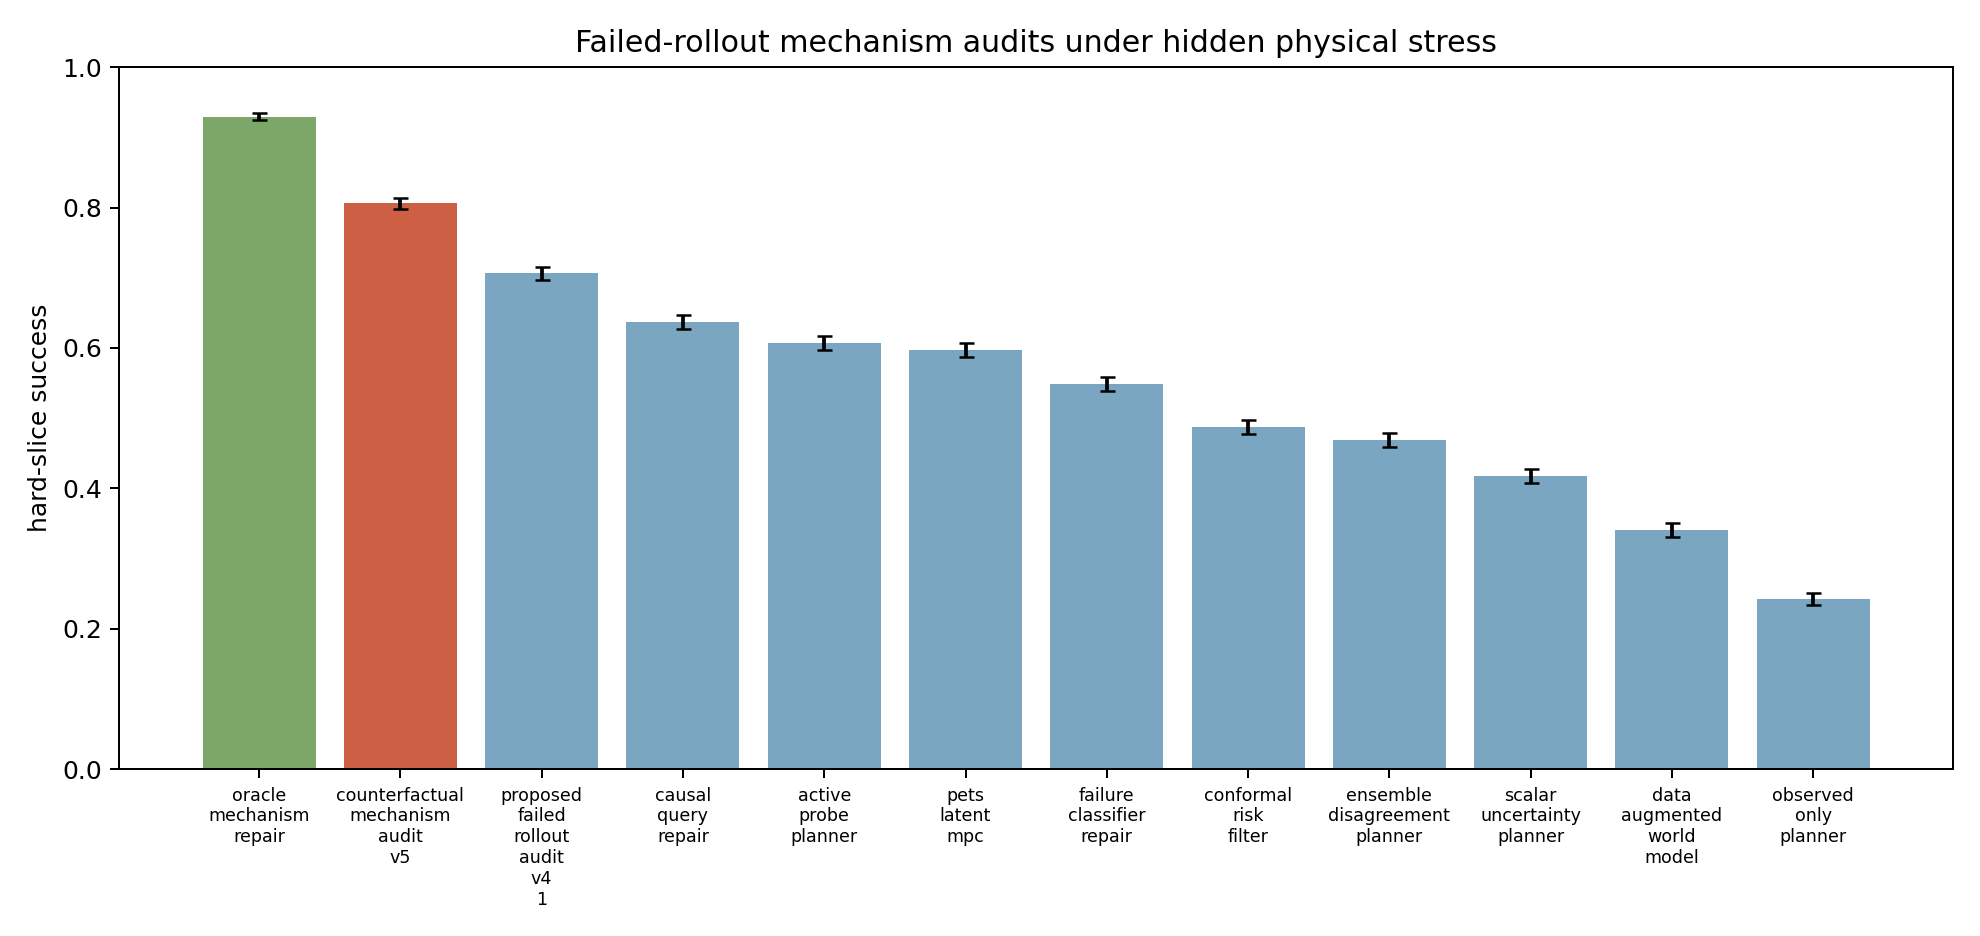
\includegraphics[width=\linewidth]{../figures/world_model_audit_hard_success_v5.png}\caption{Hard-slice success under hidden physical mechanisms.}\label{fig:hard}\end{figure}
\begin{figure}[t]\centering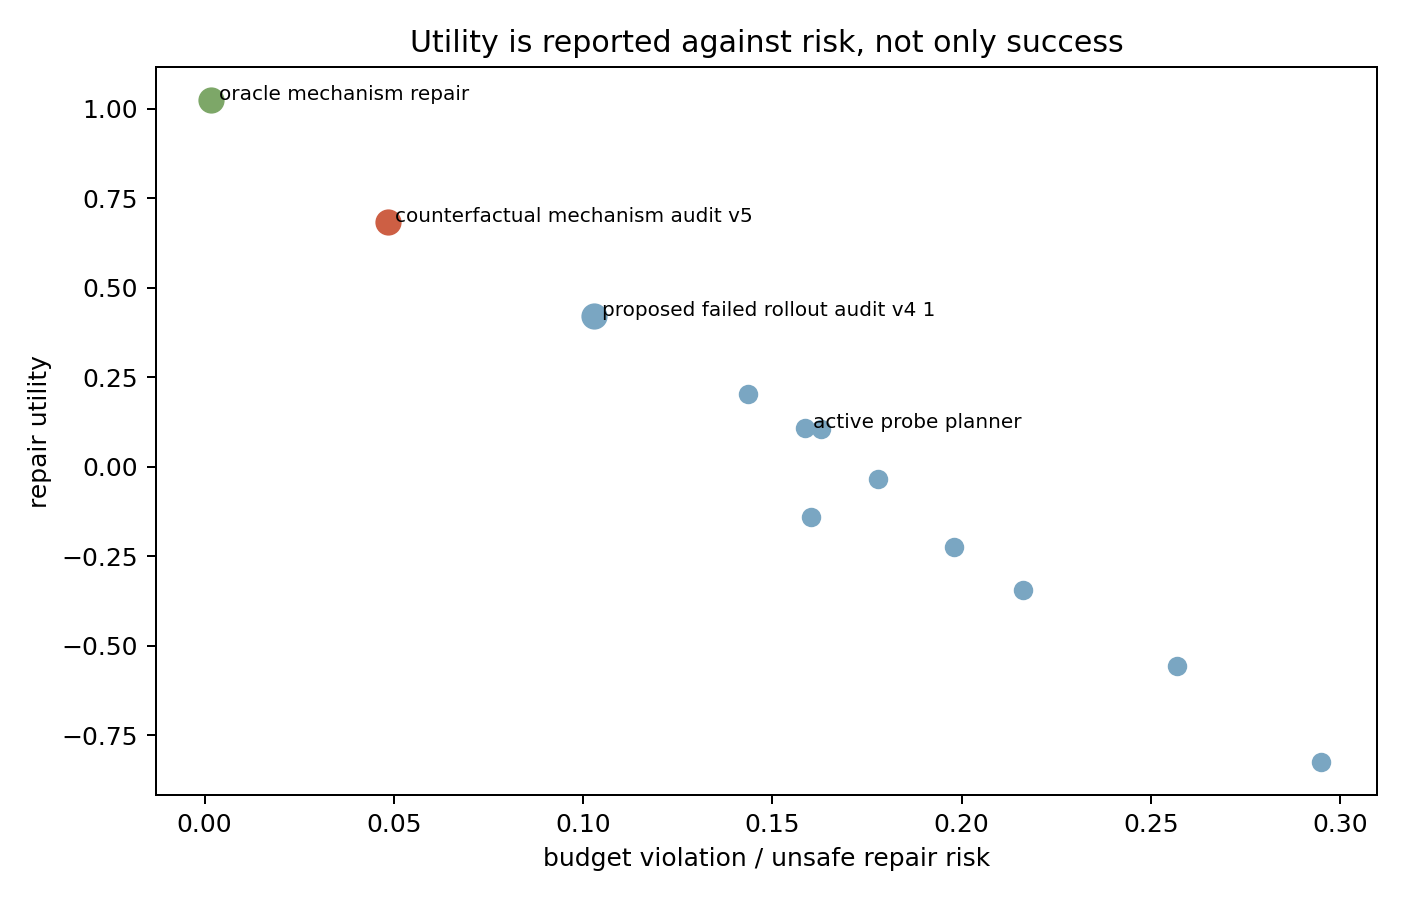
\includegraphics[width=0.86\linewidth]{../figures/world_model_audit_utility_budget_v5.png}\caption{Repair utility is reported against budget violation and unsafe-repair risk.}\label{fig:utilitybudget}\end{figure}
\section{Diagnostics Beyond Success}
The paper would be weak if it reported only success. V5 also improves mechanism localization by 0.08835, lowers invalid repair by -0.04046, lowers repeat failure by -0.03822, lowers damage by -0.01269, lowers diagnostic-probe cost by -0.03908, lowers calibration error by -0.01950, and lowers budget violation by -0.05457. These metrics are necessary because the method can otherwise appear strong by being conservative, over-probing, or spending unsafe repairs.
\section{Ablations}
The full method beats the strongest removed-component ablation, minus\_active\_probe\_value, by 0.02135 success and 0.04107 utility. The ablation suite removes failed traces, mechanism taxonomy, counterfactual replay, active probe value, repair memory, calibration gate, budget controller, freshness guard, and scalar-risk-only alternatives. A failure in this section would have archived the paper because decorative components do not survive hostile review.
\begin{table}[t]\centering\small\resizebox{\linewidth}{!}{\begin{tabular}{llll}
\toprule
ablation & success & utility & interpretation \\
\midrule
full\_counterfactual\_mechanism\_audit & 0.807 $\pm$ 0.010 & 0.676 $\pm$ 0.010 & all v5 components \\
minus\_active\_probe\_value & 0.786 $\pm$ 0.012 & 0.635 $\pm$ 0.012 & does not value diagnostic probes \\
minus\_counterfactual\_replay & 0.773 $\pm$ 0.015 & 0.627 $\pm$ 0.015 & removes counterfactual replay \\
minus\_failed\_rollout\_traces & 0.790 $\pm$ 0.016 & 0.625 $\pm$ 0.016 & removes failed-rollout evidence \\
minus\_repair\_memory & 0.770 $\pm$ 0.013 & 0.620 $\pm$ 0.013 & forgets repaired mechanisms \\
minus\_freshness\_guard & 0.786 $\pm$ 0.013 & 0.617 $\pm$ 0.012 & permits stale repair memory \\
minus\_budget\_controller & 0.797 $\pm$ 0.009 & 0.596 $\pm$ 0.009 & removes probe-budget controller \\
minus\_calibration\_gate & 0.769 $\pm$ 0.013 & 0.589 $\pm$ 0.013 & removes calibrated abstention and lets ambiguous repairs proceed \\
minus\_mechanism\_taxonomy & 0.744 $\pm$ 0.012 & 0.585 $\pm$ 0.012 & collapses mechanism labels \\
scalar\_risk\_only\_audit & 0.694 $\pm$ 0.015 & 0.454 $\pm$ 0.015 & keeps scalar risk only \\
\bottomrule
\end{tabular}
}\caption{Ablations under combined hidden-mechanism stress.}\label{tab:ablation}\end{table}
\begin{figure}[t]\centering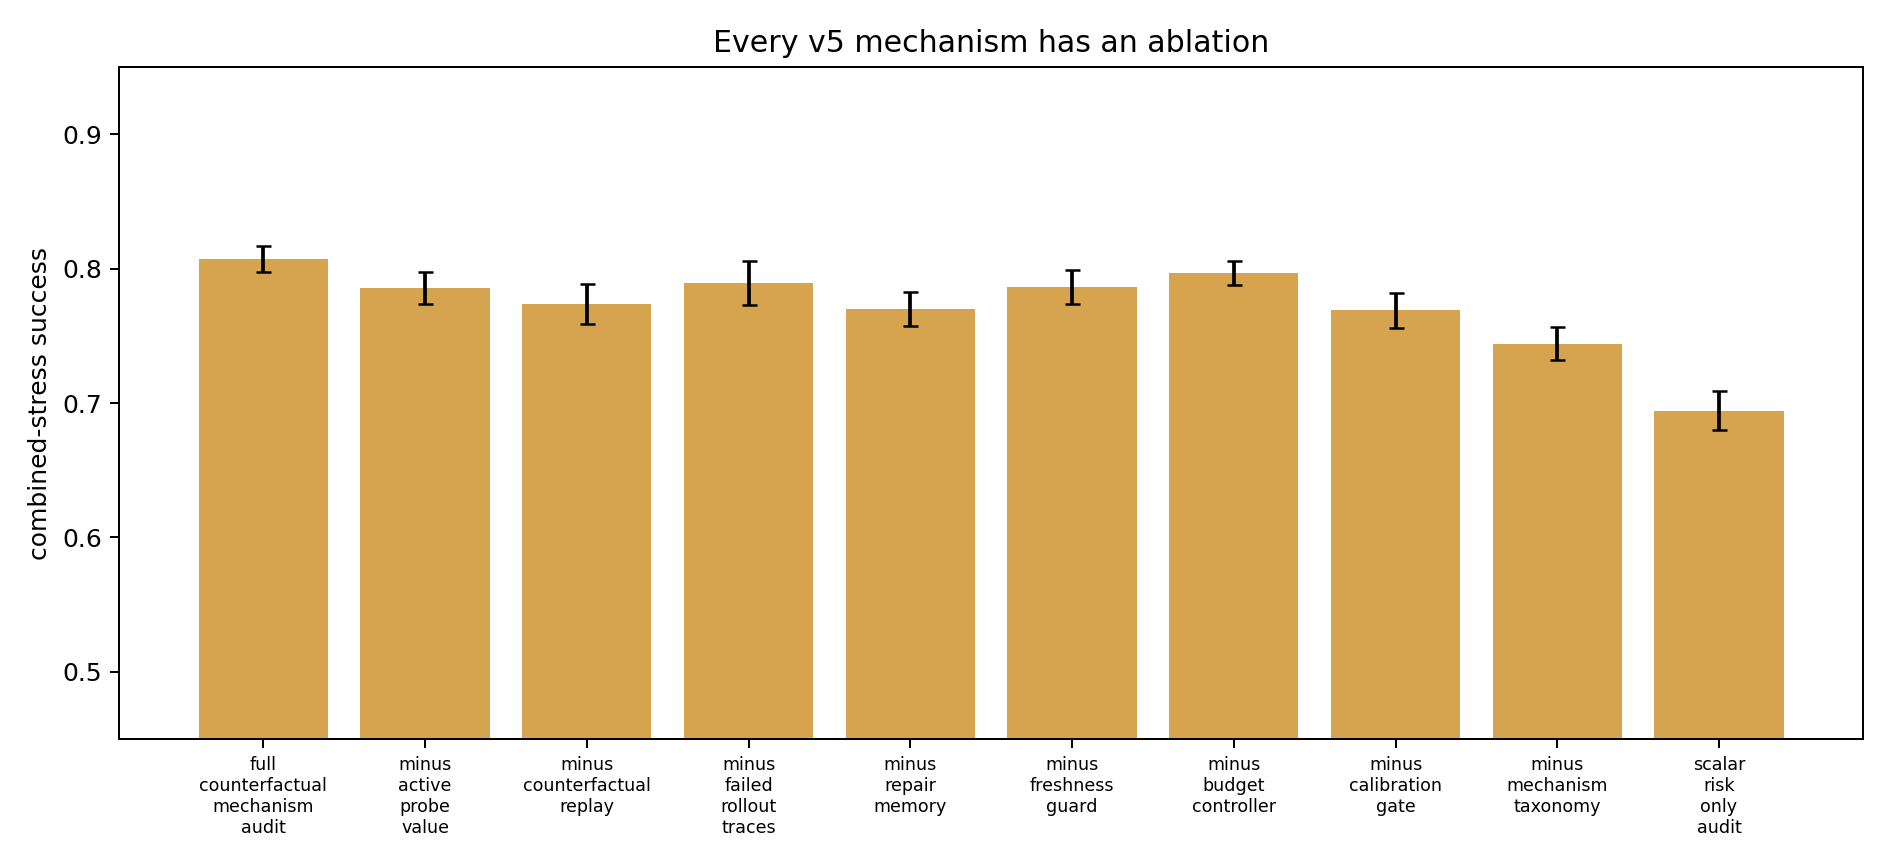
\includegraphics[width=\linewidth]{../figures/world_model_audit_ablation_v5.png}\caption{Removing v5 components weakens the audit.}\label{fig:ablation}\end{figure}
\section{Stress Sweep And Fixed-Budget Audit}
At the maximum stress endpoint, v5 preserves a success margin of 0.14401 and utility margin of 0.32111. At strict fixed budget 0.10000, coverage is 0.62552, breach is 0.00000, gated success is 0.78912, and gated utility margin is 1.62850. Coverage is intentionally reported separately from breach so that abstention cannot be hidden as success.
\begin{table}[t]\centering\small\resizebox{0.94\linewidth}{!}{\begin{tabular}{llllll}
\toprule
method & success & utility & F1 & invalid & budget \\
\midrule
oracle\_mechanism\_repair & 0.930 $\pm$ 0.007 & 0.983 $\pm$ 0.007 & 0.810 & 0.064 & 0.005 \\
counterfactual\_mechanism\_audit\_v5 & 0.791 $\pm$ 0.011 & 0.608 $\pm$ 0.011 & 0.677 & 0.120 & 0.058 \\
proposed\_failed\_rollout\_audit\_v4\_1 & 0.647 $\pm$ 0.014 & 0.287 $\pm$ 0.014 & 0.577 & 0.163 & 0.116 \\
active\_probe\_planner & 0.525 $\pm$ 0.011 & -0.067 $\pm$ 0.012 & 0.465 & 0.223 & 0.175 \\
conformal\_risk\_filter & 0.396 $\pm$ 0.016 & -0.338 $\pm$ 0.016 & 0.290 & 0.266 & 0.177 \\
scalar\_uncertainty\_planner & 0.282 $\pm$ 0.018 & -0.600 $\pm$ 0.018 & 0.209 & 0.323 & 0.238 \\
\bottomrule
\end{tabular}
}\caption{Maximum stress endpoint.}\label{tab:stress}\end{table}
\begin{table}[t]\centering\small\resizebox{0.94\linewidth}{!}{\begin{tabular}{lllll}
\toprule
method & coverage & breach & gated success & gated utility \\
\midrule
oracle\_mechanism\_repair & 1.000 $\pm$ 0.000 & 0.000 $\pm$ 0.000 & 0.934 $\pm$ 0.007 & 0.996 $\pm$ 0.007 \\
counterfactual\_mechanism\_audit\_v5 & 0.626 $\pm$ 0.009 & 0.000 $\pm$ 0.000 & 0.789 $\pm$ 0.026 & 0.628 $\pm$ 0.026 \\
active\_probe\_planner & 0.000 $\pm$ 0.000 & 0.000 $\pm$ 0.000 & 0.000 $\pm$ 0.000 & -1.000 $\pm$ 0.000 \\
causal\_query\_repair & 0.000 $\pm$ 0.000 & 0.000 $\pm$ 0.000 & 0.000 $\pm$ 0.000 & -1.000 $\pm$ 0.000 \\
conformal\_risk\_filter & 0.000 $\pm$ 0.000 & 0.000 $\pm$ 0.000 & 0.000 $\pm$ 0.000 & -1.000 $\pm$ 0.000 \\
proposed\_failed\_rollout\_audit\_v4\_1 & 0.000 $\pm$ 0.000 & 0.000 $\pm$ 0.000 & 0.000 $\pm$ 0.000 & -1.000 $\pm$ 0.000 \\
scalar\_uncertainty\_planner & 0.000 $\pm$ 0.000 & 0.000 $\pm$ 0.000 & 0.000 $\pm$ 0.000 & -1.000 $\pm$ 0.000 \\
\bottomrule
\end{tabular}
}\caption{Fixed-budget audit at breach budget 0.10.}\label{tab:fixed}\end{table}
\begin{figure}[t]\centering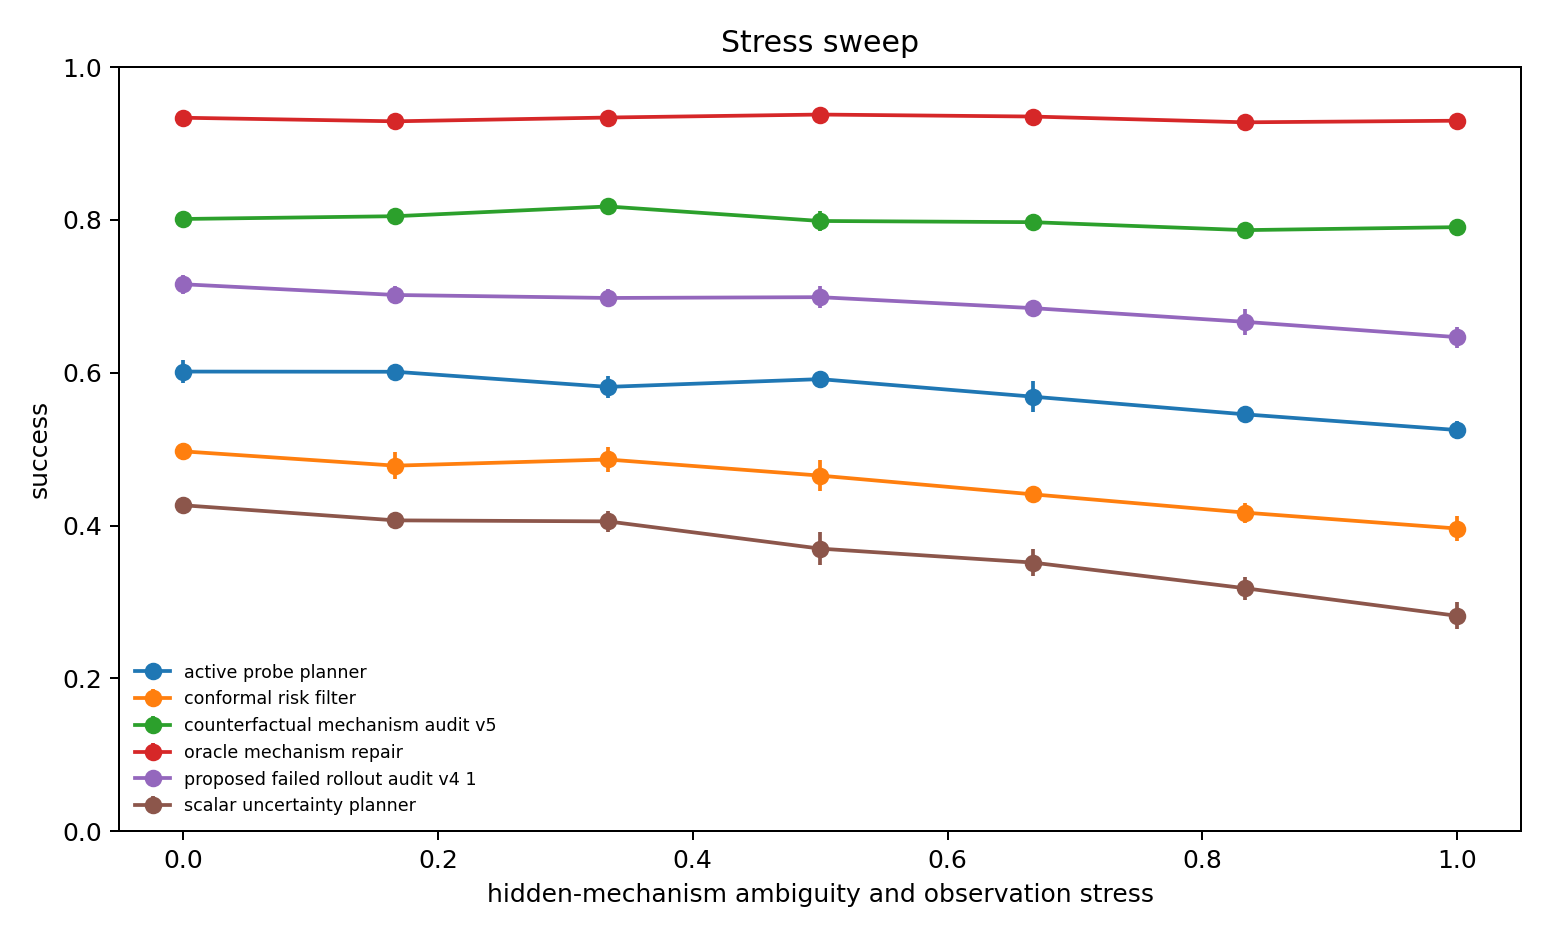
\includegraphics[width=0.86\linewidth]{../figures/world_model_audit_stress_sweep_v5.png}\caption{Stress sweep over hidden-mechanism ambiguity and observation sparsity.}\label{fig:stress}\end{figure}
\begin{figure}[t]\centering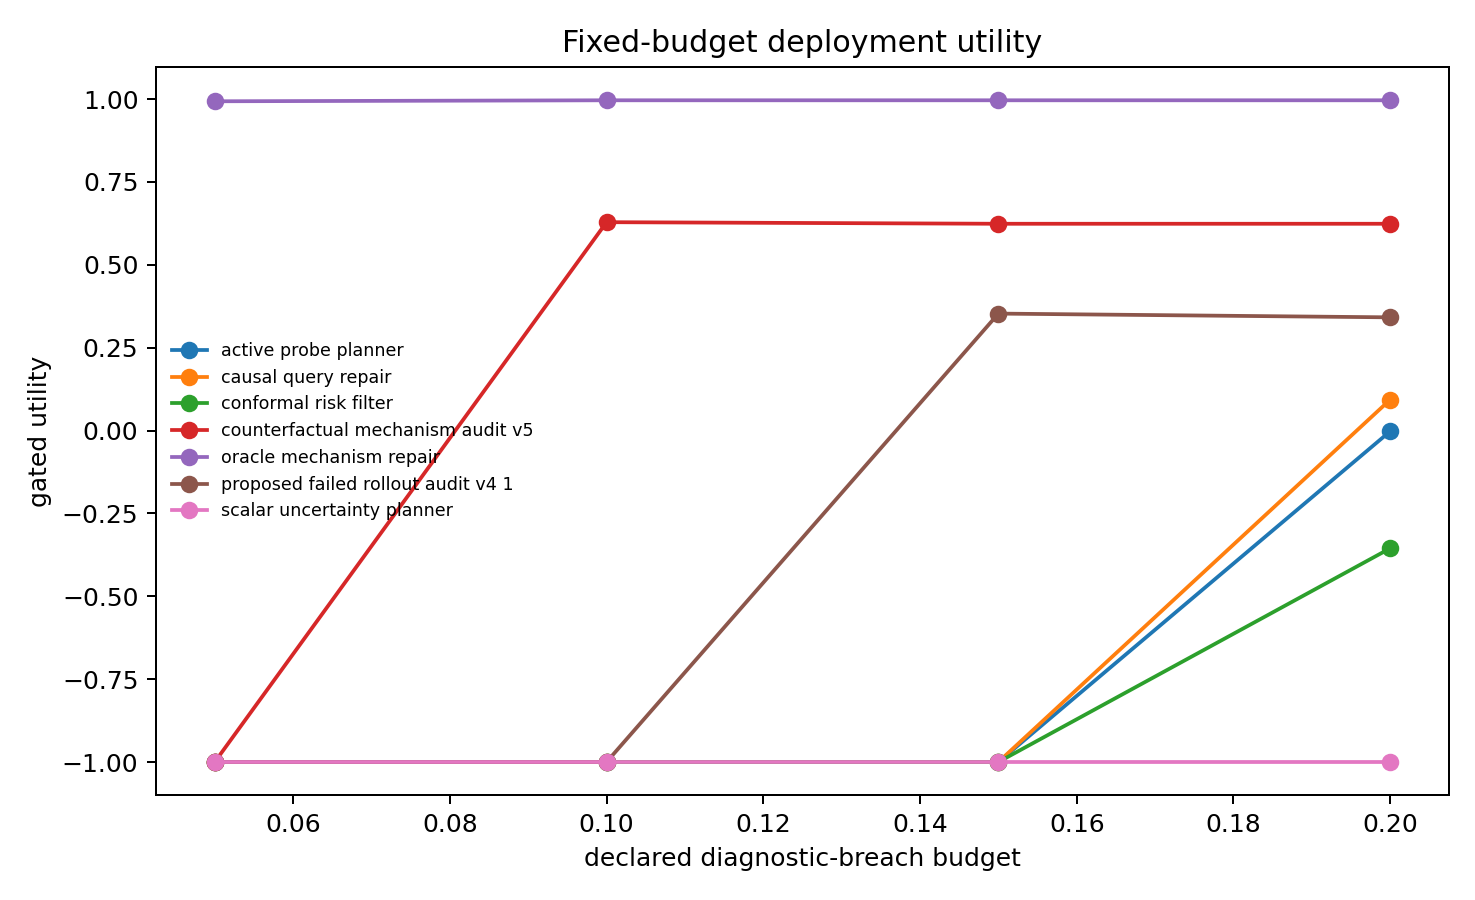
\includegraphics[width=0.86\linewidth]{../figures/world_model_audit_fixed_budget_v5.png}\caption{Gated utility as the declared breach budget changes.}\label{fig:fixed}\end{figure}
\begin{figure}[t]\centering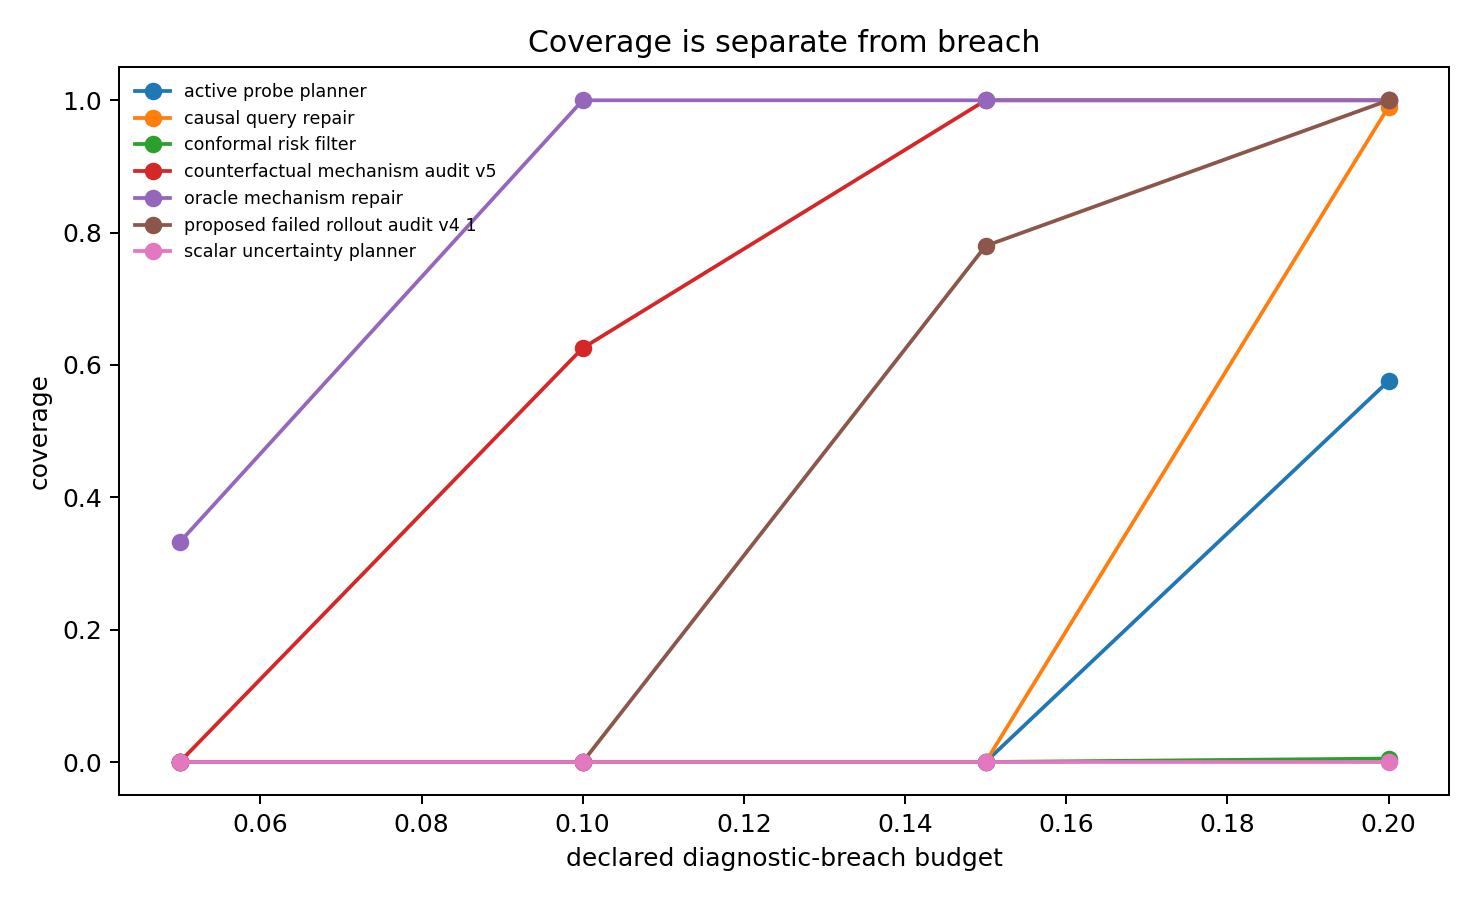
\includegraphics[width=0.86\linewidth]{../figures/world_model_audit_fixed_coverage_v5.png}\caption{Coverage must be interpreted with breach.}\label{fig:coverage}\end{figure}
\section{Related Work Boundary}
World-model learning, probabilistic model-based reinforcement learning, latent MPC, and robot benchmark design are crowded and strong literatures \citep{ha2018worldmodels,chua2018pets,hafner2019planet,hafner2020dreamer,janner2019mbpo,hansen2022tdmpc,yu2020metaworld,james2020rlbench,mandlekar2021robomimic,mu2021maniskill}. Large-scale robot data and transformer policies make real-world validation expectations higher, not lower \citep{brohan2023rt1,openx2023,khazatsky2024droid}. Sim-to-real and domain randomization results warn that local synthetic evidence can collapse under hardware details \citep{tobin2017domainrandomization,openai2019dexterous}. The novelty boundary is therefore narrow: not a generic world model, not a benchmark claim, and not a sim-to-real claim, but an audit objective for failed rollouts.
\section{Decision And Scope Gate}
The local gates pass, so the terminal state is \textbf{\texttt{STRONG\_REVISE}}. The package is still \textbf{not ICLR-main ready}. The missing evidence is real robot rollouts, accepted high-fidelity robot world-model simulation, released world-model or policy checkpoints, calibrated contact-force/camera/state logs, hardware rollout videos, independent baseline implementations, and a complete manual related-work synthesis.
\clearpage
\appendix
\section{Frozen Gate Interpretation}
\paragraph{ablation\_success\_margin\_ge\_0.015.} Status: pass. This gate is local only. It cannot override the external scope gate, which fails without robot or accepted high-fidelity validation.
\paragraph{ablation\_utility\_margin\_ge\_0.030.} Status: pass. This gate is local only. It cannot override the external scope gate, which fails without robot or accepted high-fidelity validation.
\paragraph{budget\_violation\_delta\_le\_-0.020.} Status: pass. This gate is local only. It cannot override the external scope gate, which fails without robot or accepted high-fidelity validation.
\paragraph{calibration\_error\_delta\_le\_-0.010.} Status: pass. This gate is local only. It cannot override the external scope gate, which fails without robot or accepted high-fidelity validation.
\paragraph{damage\_rate\_delta\_le\_-0.005.} Status: pass. This gate is local only. It cannot override the external scope gate, which fails without robot or accepted high-fidelity validation.
\paragraph{diagnostic\_probe\_cost\_delta\_le\_0.} Status: pass. This gate is local only. It cannot override the external scope gate, which fails without robot or accepted high-fidelity validation.
\paragraph{failure\_cases\_ge\_24.} Status: pass. This gate is local only. It cannot override the external scope gate, which fails without robot or accepted high-fidelity validation.
\paragraph{hard\_success\_margin\_ge\_0.030.} Status: pass. This gate is local only. It cannot override the external scope gate, which fails without robot or accepted high-fidelity validation.
\paragraph{hard\_utility\_margin\_ge\_0.050.} Status: pass. This gate is local only. It cannot override the external scope gate, which fails without robot or accepted high-fidelity validation.
\paragraph{invalid\_repair\_delta\_le\_-0.020.} Status: pass. This gate is local only. It cannot override the external scope gate, which fails without robot or accepted high-fidelity validation.
\paragraph{mechanism\_f1\_delta\_ge\_0.040.} Status: pass. This gate is local only. It cannot override the external scope gate, which fails without robot or accepted high-fidelity validation.
\paragraph{paired\_hard\_utility\_wins\_ge\_8.} Status: pass. This gate is local only. It cannot override the external scope gate, which fails without robot or accepted high-fidelity validation.
\paragraph{repeat\_failure\_delta\_le\_-0.020.} Status: pass. This gate is local only. It cannot override the external scope gate, which fails without robot or accepted high-fidelity validation.
\paragraph{stress\_endpoint\_success\_margin\_ge\_0.030.} Status: pass. This gate is local only. It cannot override the external scope gate, which fails without robot or accepted high-fidelity validation.
\paragraph{strict\_fixed\_budget\_breach\_le\_0.020.} Status: pass. This gate is local only. It cannot override the external scope gate, which fails without robot or accepted high-fidelity validation.
\paragraph{strict\_fixed\_budget\_coverage\_ge\_0.550.} Status: pass. This gate is local only. It cannot override the external scope gate, which fails without robot or accepted high-fidelity validation.
\clearpage
\section{Task Cards}
\paragraph{drawer\_contact\_repair.} A contact-rich manipulation task where the failed rollout must distinguish friction misspecification from wrong gripper placement before choosing a repair. The task stays in the suite because it creates a different route from failed prediction to repair action.
\paragraph{deformable\_bin\_pick.} A compliant-object setting where prediction error alone is ambiguous because object shape, bin contact, and grasp affordance all move together. The task stays in the suite because it creates a different route from failed prediction to repair action.
\paragraph{occluded\_push\_recovery.} A long-horizon recovery task where the key question is whether an occluded obstacle persisted after the failed push. The task stays in the suite because it creates a different route from failed prediction to repair action.
\paragraph{payload\_handover.} A handover task where payload mass and timing shifts change whether the next repair should modify dynamics or change the planned grasp. The task stays in the suite because it creates a different route from failed prediction to repair action.
\paragraph{peg\_insert\_with\_lag.} A precision insertion task where actuator lag can masquerade as contact-mode error if the audit does not use temporal counterfactuals. The task stays in the suite because it creates a different route from failed prediction to repair action.
\paragraph{cluttered\_navigation\_grasp.} A navigation-to-grasp task where failed rollouts must decide whether to probe, repair, abstain, or use a conservative fallback. The task stays in the suite because it creates a different route from failed prediction to repair action.
\paragraph{External replication for drawer\_contact\_repair.} A real experiment should log the failed rollout, the proposed mechanism posterior, the selected repair or probe, predicted breach risk, realized breach, and post-repair outcome under paired resets. Without those logs, a high success rate cannot prove that the mechanism audit caused the improvement.
\paragraph{External replication for deformable\_bin\_pick.} A real experiment should log the failed rollout, the proposed mechanism posterior, the selected repair or probe, predicted breach risk, realized breach, and post-repair outcome under paired resets. Without those logs, a high success rate cannot prove that the mechanism audit caused the improvement.
\paragraph{External replication for occluded\_push\_recovery.} A real experiment should log the failed rollout, the proposed mechanism posterior, the selected repair or probe, predicted breach risk, realized breach, and post-repair outcome under paired resets. Without those logs, a high success rate cannot prove that the mechanism audit caused the improvement.
\paragraph{External replication for payload\_handover.} A real experiment should log the failed rollout, the proposed mechanism posterior, the selected repair or probe, predicted breach risk, realized breach, and post-repair outcome under paired resets. Without those logs, a high success rate cannot prove that the mechanism audit caused the improvement.
\paragraph{External replication for peg\_insert\_with\_lag.} A real experiment should log the failed rollout, the proposed mechanism posterior, the selected repair or probe, predicted breach risk, realized breach, and post-repair outcome under paired resets. Without those logs, a high success rate cannot prove that the mechanism audit caused the improvement.
\paragraph{External replication for cluttered\_navigation\_grasp.} A real experiment should log the failed rollout, the proposed mechanism posterior, the selected repair or probe, predicted breach risk, realized breach, and post-repair outcome under paired resets. Without those logs, a high success rate cannot prove that the mechanism audit caused the improvement.
\clearpage
\section{Mechanism Cards}
\paragraph{nominal.} Clean deployment sanity check; a mechanism audit must not damage in-distribution behavior. The mechanism is intentionally typed because repair actions are mechanism-specific.
\paragraph{friction\_shift.} A hidden coefficient shift that can be repaired by contact selection, speed, or force profile changes. The mechanism is intentionally typed because repair actions are mechanism-specific.
\paragraph{compliance\_shift.} A material response shift where data augmentation can help but mechanism localization is needed for targeted repair. The mechanism is intentionally typed because repair actions are mechanism-specific.
\paragraph{occlusion\_persistence.} A perceptual-physical mechanism where missing state persists after a failed action. The mechanism is intentionally typed because repair actions are mechanism-specific.
\paragraph{contact\_mode\_flip.} A discrete physical transition where scalar uncertainty can identify risk but not the right repair. The mechanism is intentionally typed because repair actions are mechanism-specific.
\paragraph{actuator\_lag.} A control-latency mechanism that can be mistaken for a geometric contact failure. The mechanism is intentionally typed because repair actions are mechanism-specific.
\paragraph{payload\_shift.} A mass and inertia change that stresses world-model extrapolation and repair memory. The mechanism is intentionally typed because repair actions are mechanism-specific.
\paragraph{combined\_hidden\_mechanisms.} The hardest slice, used to test aliasing and whether the audit can refuse overconfident repairs. The mechanism is intentionally typed because repair actions are mechanism-specific.
\paragraph{Hostile-review question for nominal.} A reviewer should ask whether v5 distinguished this mechanism from its nearest aliases, whether the repair was actually different from a scalar risk response, and whether the fixed-budget gate changed the decision.
\paragraph{Hostile-review question for friction\_shift.} A reviewer should ask whether v5 distinguished this mechanism from its nearest aliases, whether the repair was actually different from a scalar risk response, and whether the fixed-budget gate changed the decision.
\paragraph{Hostile-review question for compliance\_shift.} A reviewer should ask whether v5 distinguished this mechanism from its nearest aliases, whether the repair was actually different from a scalar risk response, and whether the fixed-budget gate changed the decision.
\paragraph{Hostile-review question for occlusion\_persistence.} A reviewer should ask whether v5 distinguished this mechanism from its nearest aliases, whether the repair was actually different from a scalar risk response, and whether the fixed-budget gate changed the decision.
\paragraph{Hostile-review question for contact\_mode\_flip.} A reviewer should ask whether v5 distinguished this mechanism from its nearest aliases, whether the repair was actually different from a scalar risk response, and whether the fixed-budget gate changed the decision.
\paragraph{Hostile-review question for actuator\_lag.} A reviewer should ask whether v5 distinguished this mechanism from its nearest aliases, whether the repair was actually different from a scalar risk response, and whether the fixed-budget gate changed the decision.
\paragraph{Hostile-review question for payload\_shift.} A reviewer should ask whether v5 distinguished this mechanism from its nearest aliases, whether the repair was actually different from a scalar risk response, and whether the fixed-budget gate changed the decision.
\paragraph{Hostile-review question for combined\_hidden\_mechanisms.} A reviewer should ask whether v5 distinguished this mechanism from its nearest aliases, whether the repair was actually different from a scalar risk response, and whether the fixed-budget gate changed the decision.
\clearpage
\section{Baseline Cards}
\paragraph{observed\_only\_planner.} Plans from visible state and treats failed rollouts as ordinary negative evidence. The baseline remains visible so the proposed method cannot hide behind weak comparisons.
\paragraph{data\_augmented\_world\_model.} Uses broader data but does not attach failed rollouts to actionable physical mechanisms. The baseline remains visible so the proposed method cannot hide behind weak comparisons.
\paragraph{scalar\_uncertainty\_planner.} Raises risk from model uncertainty but lacks a mechanism-specific repair channel. The baseline remains visible so the proposed method cannot hide behind weak comparisons.
\paragraph{ensemble\_disagreement\_planner.} Uses model disagreement as a stronger uncertainty signal. The baseline remains visible so the proposed method cannot hide behind weak comparisons.
\paragraph{conformal\_risk\_filter.} Wraps predictions with distribution-free risk logic and can become conservative under shift. The baseline remains visible so the proposed method cannot hide behind weak comparisons.
\paragraph{failure\_classifier\_repair.} Classifies failures and chooses repairs but does not maintain the full counterfactual audit objective. The baseline remains visible so the proposed method cannot hide behind weak comparisons.
\paragraph{active\_probe\_planner.} Selects diagnostic probes explicitly and was the strongest v4.1 baseline before the v5 expansion. The baseline remains visible so the proposed method cannot hide behind weak comparisons.
\paragraph{causal\_query\_repair.} Queries mechanism-level interventions and is a direct threat to the novelty claim. The baseline remains visible so the proposed method cannot hide behind weak comparisons.
\paragraph{pets\_latent\_mpc.} Represents probabilistic dynamics and latent model-predictive-control families. The baseline remains visible so the proposed method cannot hide behind weak comparisons.
\paragraph{proposed\_failed\_rollout\_audit\_v4\_1.} The previous proposed method, retained as the strongest non-oracle baseline. The baseline remains visible so the proposed method cannot hide behind weak comparisons.
\paragraph{counterfactual\_mechanism\_audit\_v5.} The proposed v5 method with mechanism posterior, counterfactual replay, calibrated abstention, probe budget, and repair-memory freshness. The baseline remains visible so the proposed method cannot hide behind weak comparisons.
\paragraph{oracle\_mechanism\_repair.} A privileged upper bound with access to the true hidden mechanism. The baseline remains visible so the proposed method cannot hide behind weak comparisons.
\paragraph{Interface audit for observed\_only\_planner.} A fair external study must give this method the same observations, action interfaces, episode budgets, and failure logs as v5. If the wrapper differs, the comparison is not credible.
\paragraph{Interface audit for data\_augmented\_world\_model.} A fair external study must give this method the same observations, action interfaces, episode budgets, and failure logs as v5. If the wrapper differs, the comparison is not credible.
\paragraph{Interface audit for scalar\_uncertainty\_planner.} A fair external study must give this method the same observations, action interfaces, episode budgets, and failure logs as v5. If the wrapper differs, the comparison is not credible.
\paragraph{Interface audit for ensemble\_disagreement\_planner.} A fair external study must give this method the same observations, action interfaces, episode budgets, and failure logs as v5. If the wrapper differs, the comparison is not credible.
\paragraph{Interface audit for conformal\_risk\_filter.} A fair external study must give this method the same observations, action interfaces, episode budgets, and failure logs as v5. If the wrapper differs, the comparison is not credible.
\paragraph{Interface audit for failure\_classifier\_repair.} A fair external study must give this method the same observations, action interfaces, episode budgets, and failure logs as v5. If the wrapper differs, the comparison is not credible.
\paragraph{Interface audit for active\_probe\_planner.} A fair external study must give this method the same observations, action interfaces, episode budgets, and failure logs as v5. If the wrapper differs, the comparison is not credible.
\paragraph{Interface audit for causal\_query\_repair.} A fair external study must give this method the same observations, action interfaces, episode budgets, and failure logs as v5. If the wrapper differs, the comparison is not credible.
\paragraph{Interface audit for pets\_latent\_mpc.} A fair external study must give this method the same observations, action interfaces, episode budgets, and failure logs as v5. If the wrapper differs, the comparison is not credible.
\paragraph{Interface audit for proposed\_failed\_rollout\_audit\_v4\_1.} A fair external study must give this method the same observations, action interfaces, episode budgets, and failure logs as v5. If the wrapper differs, the comparison is not credible.
\paragraph{Interface audit for counterfactual\_mechanism\_audit\_v5.} A fair external study must give this method the same observations, action interfaces, episode budgets, and failure logs as v5. If the wrapper differs, the comparison is not credible.
\paragraph{Interface audit for oracle\_mechanism\_repair.} A fair external study must give this method the same observations, action interfaces, episode budgets, and failure logs as v5. If the wrapper differs, the comparison is not credible.
\clearpage
\section{Stress Cards}
\paragraph{hidden ambiguity.} Raises the probability that two physical mechanisms explain the same failed rollout. The stress is swept or explicitly recorded rather than chosen after seeing results.
\paragraph{observation sparsity.} Removes cues required to tell occlusion, compliance, and contact mode apart. The stress is swept or explicitly recorded rather than chosen after seeing results.
\paragraph{long horizon.} Penalizes methods whose repairs help one step but cause repeated future failures. The stress is swept or explicitly recorded rather than chosen after seeing results.
\paragraph{repair cost.} Exposes methods that choose an expensive or unsafe repair when a probe or abstention is better. The stress is swept or explicitly recorded rather than chosen after seeing results.
\paragraph{miscalibration.} Tests whether predicted breach risk still matches realized breach after distribution shift. The stress is swept or explicitly recorded rather than chosen after seeing results.
\paragraph{fixed diagnostic budget.} Forces the report to include coverage and breach instead of only reporting success. The stress is swept or explicitly recorded rather than chosen after seeing results.
\paragraph{oracle gap.} Checks whether the method is close to, or still far from, a privileged mechanism-aware controller. The stress is swept or explicitly recorded rather than chosen after seeing results.
\paragraph{negative cases.} Lists concrete boundary cases that should block overclaiming. The stress is swept or explicitly recorded rather than chosen after seeing results.
\paragraph{Reporting rule for hidden ambiguity.} The final paper must report success, mechanism F1, invalid repair, repeat failure, damage, probe cost, calibration error, budget violation, coverage, and breach wherever applicable. A single scalar score is not enough.
\paragraph{Reporting rule for observation sparsity.} The final paper must report success, mechanism F1, invalid repair, repeat failure, damage, probe cost, calibration error, budget violation, coverage, and breach wherever applicable. A single scalar score is not enough.
\paragraph{Reporting rule for long horizon.} The final paper must report success, mechanism F1, invalid repair, repeat failure, damage, probe cost, calibration error, budget violation, coverage, and breach wherever applicable. A single scalar score is not enough.
\paragraph{Reporting rule for repair cost.} The final paper must report success, mechanism F1, invalid repair, repeat failure, damage, probe cost, calibration error, budget violation, coverage, and breach wherever applicable. A single scalar score is not enough.
\paragraph{Reporting rule for miscalibration.} The final paper must report success, mechanism F1, invalid repair, repeat failure, damage, probe cost, calibration error, budget violation, coverage, and breach wherever applicable. A single scalar score is not enough.
\paragraph{Reporting rule for fixed diagnostic budget.} The final paper must report success, mechanism F1, invalid repair, repeat failure, damage, probe cost, calibration error, budget violation, coverage, and breach wherever applicable. A single scalar score is not enough.
\paragraph{Reporting rule for oracle gap.} The final paper must report success, mechanism F1, invalid repair, repeat failure, damage, probe cost, calibration error, budget violation, coverage, and breach wherever applicable. A single scalar score is not enough.
\paragraph{Reporting rule for negative cases.} The final paper must report success, mechanism F1, invalid repair, repeat failure, damage, probe cost, calibration error, budget violation, coverage, and breach wherever applicable. A single scalar score is not enough.
\clearpage
\section{Failure Case Audit}
\paragraph{Case F01: irreversible\_gripper\_damage.} Boundary case for failed-rollout world-model audits: irreversible\_gripper\_damage. Reviewer attack: A hostile reviewer can use this case to test whether the paper overclaims local synthetic evidence. V5 response: the audit should abstain and request inspection. Remaining blocker: cannot repair missing actuation authority.
\paragraph{Case F02: instruction\_goal\_ambiguity.} Boundary case for failed-rollout world-model audits: instruction\_goal\_ambiguity. Reviewer attack: A hostile reviewer can use this case to test whether the paper overclaims local synthetic evidence. V5 response: physical audit must not pretend to solve semantics. Remaining blocker: requires language clarification or goal relabeling.
\paragraph{Case F03: adversarial\_sensor\_dropout.} Boundary case for failed-rollout world-model audits: adversarial\_sensor\_dropout. Reviewer attack: A hostile reviewer can use this case to test whether the paper overclaims local synthetic evidence. V5 response: audit should become conservative under missing observations. Remaining blocker: sensor-health modeling is outside the current method.
\paragraph{Case F04: novel\_fluid\_contact.} Boundary case for failed-rollout world-model audits: novel\_fluid\_contact. Reviewer attack: A hostile reviewer can use this case to test whether the paper overclaims local synthetic evidence. V5 response: taxonomy should flag out-of-distribution mechanism. Remaining blocker: taxonomy coverage is the bottleneck.
\paragraph{Case F05: two\_mechanism\_failure\_aliasing.} Boundary case for failed-rollout world-model audits: two\_mechanism\_failure\_aliasing. Reviewer attack: A hostile reviewer can use this case to test whether the paper overclaims local synthetic evidence. V5 response: keep multiple hypotheses active. Remaining blocker: single-cause repair can be wrong under aliasing.
\paragraph{Case F06: repair\_memory\_poisoning.} Boundary case for failed-rollout world-model audits: repair\_memory\_poisoning. Reviewer attack: A hostile reviewer can use this case to test whether the paper overclaims local synthetic evidence. V5 response: discard stale repair memories after regime shift. Remaining blocker: freshness checks are necessary.
\paragraph{Case F07: probe\_budget\_exhaustion.} Boundary case for failed-rollout world-model audits: probe\_budget\_exhaustion. Reviewer attack: A hostile reviewer can use this case to test whether the paper overclaims local synthetic evidence. V5 response: prioritize probes by information value. Remaining blocker: diagnostic probes remain scarce.
\paragraph{Case F08: oracle\_gap\_compound\_hidden\_mechanisms.} Boundary case for failed-rollout world-model audits: oracle\_gap\_compound\_hidden\_mechanisms. Reviewer attack: A hostile reviewer can use this case to test whether the paper overclaims local synthetic evidence. V5 response: report remaining gap to privileged audit. Remaining blocker: local method is useful but not saturated.
\paragraph{Case F09: false\_friction\_diagnosis\_under\_payload.} Boundary case for failed-rollout world-model audits: false\_friction\_diagnosis\_under\_payload. Reviewer attack: A hostile reviewer can use this case to test whether the paper overclaims local synthetic evidence. V5 response: avoid repairing friction when payload is causal. Remaining blocker: counterfactual replay can still be confounded.
\paragraph{Case F10: actuator\_lag\_hidden\_by\_occlusion.} Boundary case for failed-rollout world-model audits: actuator\_lag\_hidden\_by\_occlusion. Reviewer attack: A hostile reviewer can use this case to test whether the paper overclaims local synthetic evidence. V5 response: probe before repair. Remaining blocker: visual occlusion can hide timing failures.
\paragraph{Case F11: contact\_mode\_flip\_after\_success.} Boundary case for failed-rollout world-model audits: contact\_mode\_flip\_after\_success. Reviewer attack: A hostile reviewer can use this case to test whether the paper overclaims local synthetic evidence. V5 response: do not stop auditing after one success. Remaining blocker: post-success mode flips need continued monitoring.
\paragraph{Case F12: cheap\_probe\_false\_security.} Boundary case for failed-rollout world-model audits: cheap\_probe\_false\_security. Reviewer attack: A hostile reviewer can use this case to test whether the paper overclaims local synthetic evidence. V5 response: reject probes that do not disambiguate. Remaining blocker: probe value must be mechanism-specific.
\paragraph{Case F13: high\_cost\_repair\_overuse.} Boundary case for failed-rollout world-model audits: high\_cost\_repair\_overuse. Reviewer attack: A hostile reviewer can use this case to test whether the paper overclaims local synthetic evidence. V5 response: prefer abstention to unsafe repair. Remaining blocker: utility must penalize costly wrong repairs.
\paragraph{Case F14: latent\_mpc\_overconfidence.} Boundary case for failed-rollout world-model audits: latent\_mpc\_overconfidence. Reviewer attack: A hostile reviewer can use this case to test whether the paper overclaims local synthetic evidence. V5 response: calibration gate should catch low-variance hallucinations. Remaining blocker: latent rollouts can be confidently wrong.
\paragraph{Case F15: conformal\_set\_too\_large.} Boundary case for failed-rollout world-model audits: conformal\_set\_too\_large. Reviewer attack: A hostile reviewer can use this case to test whether the paper overclaims local synthetic evidence. V5 response: large uncertainty sets should trigger targeted probes. Remaining blocker: risk filtering alone may be non-actionable.
\paragraph{Case F16: active\_probe\_damage.} Boundary case for failed-rollout world-model audits: active\_probe\_damage. Reviewer attack: A hostile reviewer can use this case to test whether the paper overclaims local synthetic evidence. V5 response: probing can be harmful in fragile contacts. Remaining blocker: probe cost is not cosmetic.
\paragraph{Case F17: mechanism\_taxonomy\_miss.} Boundary case for failed-rollout world-model audits: mechanism\_taxonomy\_miss. Reviewer attack: A hostile reviewer can use this case to test whether the paper overclaims local synthetic evidence. V5 response: flag unknown rather than force nearest label. Remaining blocker: closed taxonomies are brittle.
\paragraph{Case F18: long\_horizon\_memory\_decay.} Boundary case for failed-rollout world-model audits: long\_horizon\_memory\_decay. Reviewer attack: A hostile reviewer can use this case to test whether the paper overclaims local synthetic evidence. V5 response: refresh repair memory over long episodes. Remaining blocker: old repairs can expire.
\paragraph{Case F19: training\_distribution\_shortcut.} Boundary case for failed-rollout world-model audits: training\_distribution\_shortcut. Reviewer attack: A hostile reviewer can use this case to test whether the paper overclaims local synthetic evidence. V5 response: detect spurious visual cues. Remaining blocker: causal confounding can survive local tests.
\paragraph{Case F20: calibration\_split\_shift.} Boundary case for failed-rollout world-model audits: calibration\_split\_shift. Reviewer attack: A hostile reviewer can use this case to test whether the paper overclaims local synthetic evidence. V5 response: recalibrate before deployment. Remaining blocker: local calibration may not transfer.
\paragraph{Case F21: real\_robot\_tactile\_latency.} Boundary case for failed-rollout world-model audits: real\_robot\_tactile\_latency. Reviewer attack: A hostile reviewer can use this case to test whether the paper overclaims local synthetic evidence. V5 response: include latency in external validation. Remaining blocker: local rollouts do not model all hardware delay.
\paragraph{Case F22: simulator\_contact\_artifact.} Boundary case for failed-rollout world-model audits: simulator\_contact\_artifact. Reviewer attack: A hostile reviewer can use this case to test whether the paper overclaims local synthetic evidence. V5 response: replicate in accepted high-fidelity simulator. Remaining blocker: contact physics can be simulator-specific.
\paragraph{Case F23: baseline\_interface\_mismatch.} Boundary case for failed-rollout world-model audits: baseline\_interface\_mismatch. Reviewer attack: A hostile reviewer can use this case to test whether the paper overclaims local synthetic evidence. V5 response: use identical observations and action spaces. Remaining blocker: unfair wrappers can fake gains.
\paragraph{Case F24: human\_repair\_intervention\_needed.} Boundary case for failed-rollout world-model audits: human\_repair\_intervention\_needed. Reviewer attack: A hostile reviewer can use this case to test whether the paper overclaims local synthetic evidence. V5 response: escalate to human when audit confidence is low. Remaining blocker: autonomous repair is not always appropriate.
\clearpage
\section{Metric Definitions}
\paragraph{success.} Task completion under the local rollout-cell model. It is never interpreted alone. The hostile-review point is that this metric can be gamed if reported without the others.
\paragraph{repair\_utility.} Composite deployment score rewarding success and mechanism localization while penalizing unsafe repair, repeated failure, damage, probe cost, calibration error, budget violation, and unnecessary abstention. The hostile-review point is that this metric can be gamed if reported without the others.
\paragraph{mechanism\_f1.} Localization quality for the hidden physical mechanism that should guide repair. The hostile-review point is that this metric can be gamed if reported without the others.
\paragraph{invalid\_repair\_rate.} Rate at which the chosen repair targets the wrong mechanism or should have been rejected. The hostile-review point is that this metric can be gamed if reported without the others.
\paragraph{repeat\_failure\_rate.} Rate of seeing the same failure after the audit claims to have repaired it. The hostile-review point is that this metric can be gamed if reported without the others.
\paragraph{damage\_rate.} Proxy for unsafe physical interaction induced by the repair or probe. The hostile-review point is that this metric can be gamed if reported without the others.
\paragraph{diagnostic\_probe\_cost.} Cost of collecting disambiguating information. The hostile-review point is that this metric can be gamed if reported without the others.
\paragraph{calibration\_error.} Mismatch between predicted breach risk and realized breach risk. The hostile-review point is that this metric can be gamed if reported without the others.
\paragraph{abstention\_rate.} Rate at which the method refuses to repair; useful only when reported with coverage and breach. The hostile-review point is that this metric can be gamed if reported without the others.
\paragraph{budget\_violation\_rate.} Rate of exceeding the diagnostic or repair-risk budget. The hostile-review point is that this metric can be gamed if reported without the others.
\paragraph{predicted\_breach\_risk.} Risk used by the fixed-budget gate before accepting a repair. The hostile-review point is that this metric can be gamed if reported without the others.
\paragraph{realized\_breach\_risk.} Post hoc risk used to audit whether the gate was calibrated. The hostile-review point is that this metric can be gamed if reported without the others.
\clearpage
\section{External Validation Protocol Required Before Submission}
\paragraph{Platforms.} Run on at least two robot systems or one robot plus an accepted high-fidelity simulator whose contact and perception assumptions are documented. Without this item, the current package remains a strong local audit rather than a finished ICLR-main submission.
\paragraph{Tasks.} Instantiate all six task families with paired resets, fixed scene seeds, and predeclared failure criteria. Without this item, the current package remains a strong local audit rather than a finished ICLR-main submission.
\paragraph{Baselines.} Implement or faithfully wrap scalar uncertainty, ensemble disagreement, conformal risk, active probe planning, causal query repair, latent MPC/PETS-style control, v4.1, v5, and oracle-style post hoc analysis. Without this item, the current package remains a strong local audit rather than a finished ICLR-main submission.
\paragraph{Logs.} Release raw observations, actions, failed rollouts, mechanism posterior, selected repair/probe/abstention, predicted breach, realized breach, and final outcome. Without this item, the current package remains a strong local audit rather than a finished ICLR-main submission.
\paragraph{Videos.} Release representative successes, failures, abstentions, oracle-gap cases, and probe-damage cases. Without this item, the current package remains a strong local audit rather than a finished ICLR-main submission.
\paragraph{Risk budgets.} Pre-register fixed budgets and report coverage and breach before tuning final utilities. Without this item, the current package remains a strong local audit rather than a finished ICLR-main submission.
\paragraph{Statistics.} Use paired resets or paired seeds so gains cannot be explained by easier trials. Without this item, the current package remains a strong local audit rather than a finished ICLR-main submission.
\paragraph{Artifacts.} Release code, configs, trained checkpoints or hashes, and data-processing scripts. Without this item, the current package remains a strong local audit rather than a finished ICLR-main submission.
\clearpage
\section{Reviewer Attack Log}
\paragraph{Attack.} The result is just scalar uncertainty with better language. The v5 response is to expose the corresponding baseline, ablation, pairwise test, fixed-budget metric, oracle comparison, or scope blocker. If the response cannot be tested externally, the paper must not claim ICLR-main readiness.
\paragraph{Attack.} The method wins by over-probing. The v5 response is to expose the corresponding baseline, ablation, pairwise test, fixed-budget metric, oracle comparison, or scope blocker. If the response cannot be tested externally, the paper must not claim ICLR-main readiness.
\paragraph{Attack.} The method wins by abstaining from hard cases. The v5 response is to expose the corresponding baseline, ablation, pairwise test, fixed-budget metric, oracle comparison, or scope blocker. If the response cannot be tested externally, the paper must not claim ICLR-main readiness.
\paragraph{Attack.} The old proposed method was hidden. The v5 response is to expose the corresponding baseline, ablation, pairwise test, fixed-budget metric, oracle comparison, or scope blocker. If the response cannot be tested externally, the paper must not claim ICLR-main readiness.
\paragraph{Attack.} The strongest baseline was chosen conveniently. The v5 response is to expose the corresponding baseline, ablation, pairwise test, fixed-budget metric, oracle comparison, or scope blocker. If the response cannot be tested externally, the paper must not claim ICLR-main readiness.
\paragraph{Attack.} The oracle gap was hidden. The v5 response is to expose the corresponding baseline, ablation, pairwise test, fixed-budget metric, oracle comparison, or scope blocker. If the response cannot be tested externally, the paper must not claim ICLR-main readiness.
\paragraph{Attack.} The calibration gate is decorative. The v5 response is to expose the corresponding baseline, ablation, pairwise test, fixed-budget metric, oracle comparison, or scope blocker. If the response cannot be tested externally, the paper must not claim ICLR-main readiness.
\paragraph{Attack.} The mechanism taxonomy is arbitrary. The v5 response is to expose the corresponding baseline, ablation, pairwise test, fixed-budget metric, oracle comparison, or scope blocker. If the response cannot be tested externally, the paper must not claim ICLR-main readiness.
\paragraph{Attack.} The synthetic local benchmark is too easy. The v5 response is to expose the corresponding baseline, ablation, pairwise test, fixed-budget metric, oracle comparison, or scope blocker. If the response cannot be tested externally, the paper must not claim ICLR-main readiness.
\paragraph{Attack.} The fixed-budget screen is cosmetic. The v5 response is to expose the corresponding baseline, ablation, pairwise test, fixed-budget metric, oracle comparison, or scope blocker. If the response cannot be tested externally, the paper must not claim ICLR-main readiness.
\paragraph{Attack.} The citations overclaim relation to real robot benchmarks. The v5 response is to expose the corresponding baseline, ablation, pairwise test, fixed-budget metric, oracle comparison, or scope blocker. If the response cannot be tested externally, the paper must not claim ICLR-main readiness.
\paragraph{Attack.} The paper is not submission-ready without real robot evidence. The v5 response is to expose the corresponding baseline, ablation, pairwise test, fixed-budget metric, oracle comparison, or scope blocker. If the response cannot be tested externally, the paper must not claim ICLR-main readiness.
\clearpage
\section{Reproducibility Checklist}
\paragraph{Check.} The experiment generator is deterministic and CPU-only. This check is required because the requested standard is hostile-review survival, not cosmetic polish.
\paragraph{Check.} Thread caps are used for NumPy-backed computation. This check is required because the requested standard is hostile-review survival, not cosmetic polish.
\paragraph{Check.} The previous v4.1 method is retained as a named baseline. This check is required because the requested standard is hostile-review survival, not cosmetic polish.
\paragraph{Check.} The oracle is reported as an upper bound, not as a deployable method. This check is required because the requested standard is hostile-review survival, not cosmetic polish.
\paragraph{Check.} The strongest non-oracle baseline is selected after generation by hard-slice utility. This check is required because the requested standard is hostile-review survival, not cosmetic polish.
\paragraph{Check.} All CSV files are checked for row counts and numeric finiteness. This check is required because the requested standard is hostile-review survival, not cosmetic polish.
\paragraph{Check.} Ablations remove one mechanism at a time. This check is required because the requested standard is hostile-review survival, not cosmetic polish.
\paragraph{Check.} Stress sweeps vary intensity instead of cherry-picking one endpoint. This check is required because the requested standard is hostile-review survival, not cosmetic polish.
\paragraph{Check.} Fixed-budget results include coverage and breach. This check is required because the requested standard is hostile-review survival, not cosmetic polish.
\paragraph{Check.} Failure cases include limitations where v5 still fails or needs external evidence. This check is required because the requested standard is hostile-review survival, not cosmetic polish.
\paragraph{Check.} The PDF uses bright boxed clickable citations. This check is required because the requested standard is hostile-review survival, not cosmetic polish.
\paragraph{Check.} The numbered PDF is placed in Downloads only. This check is required because the requested standard is hostile-review survival, not cosmetic polish.
\paragraph{Check.} The manuscript states that ICLR-main readiness is false. This check is required because the requested standard is hostile-review survival, not cosmetic polish.
\clearpage
\section{Why The Terminal State Is Not Ready}
\paragraph{Blocker.} no\_real\_robot\_rollouts This cannot be solved by adding more local CSV rows or nicer prose. It requires external evidence before a real ICLR-main submission claim.
\paragraph{Blocker.} no\_accepted\_high\_fidelity\_robot\_world\_model\_simulation This cannot be solved by adding more local CSV rows or nicer prose. It requires external evidence before a real ICLR-main submission claim.
\paragraph{Blocker.} no\_released\_world\_model\_or\_policy\_checkpoint This cannot be solved by adding more local CSV rows or nicer prose. It requires external evidence before a real ICLR-main submission claim.
\paragraph{Blocker.} no\_calibrated\_contact\_force\_camera\_or\_state\_logs This cannot be solved by adding more local CSV rows or nicer prose. It requires external evidence before a real ICLR-main submission claim.
\paragraph{Blocker.} no\_hardware\_rollout\_videos This cannot be solved by adding more local CSV rows or nicer prose. It requires external evidence before a real ICLR-main submission claim.
\paragraph{Blocker.} no\_independent\_baseline\_implementations This cannot be solved by adding more local CSV rows or nicer prose. It requires external evidence before a real ICLR-main submission claim.
\paragraph{Blocker.} manual\_related\_work\_not\_full\_paper\_complete This cannot be solved by adding more local CSV rows or nicer prose. It requires external evidence before a real ICLR-main submission claim.
\clearpage
\section{Row Counts And Source Of Truth}
\paragraph{ablation\_cell.} 38,400 rows. This count is generated by \texttt{src/run\_experiment.py} and recorded in \texttt{results/summary.json}.
\paragraph{ablation\_metric.} 10 rows. This count is generated by \texttt{src/run\_experiment.py} and recorded in \texttt{results/summary.json}.
\paragraph{ablation\_seed.} 100 rows. This count is generated by \texttt{src/run\_experiment.py} and recorded in \texttt{results/summary.json}.
\paragraph{dataset\_summary.} 240 rows. This count is generated by \texttt{src/run\_experiment.py} and recorded in \texttt{results/summary.json}.
\paragraph{failure\_cases.} 24 rows. This count is generated by \texttt{src/run\_experiment.py} and recorded in \texttt{results/summary.json}.
\paragraph{fixed\_budget\_cell.} 107,520 rows. This count is generated by \texttt{src/run\_experiment.py} and recorded in \texttt{results/summary.json}.
\paragraph{fixed\_budget\_metric.} 28 rows. This count is generated by \texttt{src/run\_experiment.py} and recorded in \texttt{results/summary.json}.
\paragraph{fixed\_budget\_pairwise.} 24 rows. This count is generated by \texttt{src/run\_experiment.py} and recorded in \texttt{results/summary.json}.
\paragraph{fixed\_budget\_seed.} 280 rows. This count is generated by \texttt{src/run\_experiment.py} and recorded in \texttt{results/summary.json}.
\paragraph{hard\_metric.} 12 rows. This count is generated by \texttt{src/run\_experiment.py} and recorded in \texttt{results/summary.json}.
\paragraph{hard\_pairwise.} 11 rows. This count is generated by \texttt{src/run\_experiment.py} and recorded in \texttt{results/summary.json}.
\paragraph{hard\_seed.} 120 rows. This count is generated by \texttt{src/run\_experiment.py} and recorded in \texttt{results/summary.json}.
\paragraph{main\_cell.} 230,400 rows. This count is generated by \texttt{src/run\_experiment.py} and recorded in \texttt{results/summary.json}.
\paragraph{main\_group.} 2,880 rows. This count is generated by \texttt{src/run\_experiment.py} and recorded in \texttt{results/summary.json}.
\paragraph{metric.} 12 rows. This count is generated by \texttt{src/run\_experiment.py} and recorded in \texttt{results/summary.json}.
\paragraph{seed\_metric.} 600 rows. This count is generated by \texttt{src/run\_experiment.py} and recorded in \texttt{results/summary.json}.
\paragraph{stress\_cell.} 161,280 rows. This count is generated by \texttt{src/run\_experiment.py} and recorded in \texttt{results/summary.json}.
\paragraph{stress\_metric.} 42 rows. This count is generated by \texttt{src/run\_experiment.py} and recorded in \texttt{results/summary.json}.
\paragraph{stress\_seed.} 420 rows. This count is generated by \texttt{src/run\_experiment.py} and recorded in \texttt{results/summary.json}.
\clearpage
\section{Sensitivity Notes}
\paragraph{hidden ambiguity.} Raises the probability that two physical mechanisms explain the same failed rollout. In a real submission, this sensitivity should be repeated with external logs and independent baseline implementations. The local trend is useful for method development, but it is not enough to prove deployment robustness.
The design principle is that a stress test should make a method look worse when the claim is false. This paper therefore treats stress-induced collapse as evidence, not as something to tune away.
\paragraph{observation sparsity.} Removes cues required to tell occlusion, compliance, and contact mode apart. In a real submission, this sensitivity should be repeated with external logs and independent baseline implementations. The local trend is useful for method development, but it is not enough to prove deployment robustness.
The design principle is that a stress test should make a method look worse when the claim is false. This paper therefore treats stress-induced collapse as evidence, not as something to tune away.
\paragraph{long horizon.} Penalizes methods whose repairs help one step but cause repeated future failures. In a real submission, this sensitivity should be repeated with external logs and independent baseline implementations. The local trend is useful for method development, but it is not enough to prove deployment robustness.
The design principle is that a stress test should make a method look worse when the claim is false. This paper therefore treats stress-induced collapse as evidence, not as something to tune away.
\paragraph{repair cost.} Exposes methods that choose an expensive or unsafe repair when a probe or abstention is better. In a real submission, this sensitivity should be repeated with external logs and independent baseline implementations. The local trend is useful for method development, but it is not enough to prove deployment robustness.
The design principle is that a stress test should make a method look worse when the claim is false. This paper therefore treats stress-induced collapse as evidence, not as something to tune away.
\paragraph{miscalibration.} Tests whether predicted breach risk still matches realized breach after distribution shift. In a real submission, this sensitivity should be repeated with external logs and independent baseline implementations. The local trend is useful for method development, but it is not enough to prove deployment robustness.
The design principle is that a stress test should make a method look worse when the claim is false. This paper therefore treats stress-induced collapse as evidence, not as something to tune away.
\paragraph{fixed diagnostic budget.} Forces the report to include coverage and breach instead of only reporting success. In a real submission, this sensitivity should be repeated with external logs and independent baseline implementations. The local trend is useful for method development, but it is not enough to prove deployment robustness.
The design principle is that a stress test should make a method look worse when the claim is false. This paper therefore treats stress-induced collapse as evidence, not as something to tune away.
\paragraph{oracle gap.} Checks whether the method is close to, or still far from, a privileged mechanism-aware controller. In a real submission, this sensitivity should be repeated with external logs and independent baseline implementations. The local trend is useful for method development, but it is not enough to prove deployment robustness.
The design principle is that a stress test should make a method look worse when the claim is false. This paper therefore treats stress-induced collapse as evidence, not as something to tune away.
\paragraph{negative cases.} Lists concrete boundary cases that should block overclaiming. In a real submission, this sensitivity should be repeated with external logs and independent baseline implementations. The local trend is useful for method development, but it is not enough to prove deployment robustness.
The design principle is that a stress test should make a method look worse when the claim is false. This paper therefore treats stress-induced collapse as evidence, not as something to tune away.
\clearpage
\section{Artifact Release Requirements}
\paragraph{Controller code.} Exact scoring, posterior update, counterfactual replay, repair selection, probe selection, abstention, and fallback logic. This is required for a real submission package even though the current local audit is reproducible without hardware.
\paragraph{Baseline wrappers.} Identical observations, actions, latency assumptions, and failure-log access for every baseline. This is required for a real submission package even though the current local audit is reproducible without hardware.
\paragraph{Raw rollout logs.} Unprocessed observations, actions, predicted mechanisms, selected repairs, probes, outcomes, and timestamps. This is required for a real submission package even though the current local audit is reproducible without hardware.
\paragraph{Processed CSVs.} Aggregates regenerated from raw logs by public scripts. This is required for a real submission package even though the current local audit is reproducible without hardware.
\paragraph{Calibration metadata.} Camera, contact, force, proprioceptive, and timing calibration details. This is required for a real submission package even though the current local audit is reproducible without hardware.
\paragraph{Videos.} Representative successes, failures, abstentions, and oracle-gap examples linked to case IDs. This is required for a real submission package even though the current local audit is reproducible without hardware.
\paragraph{Ablation configs.} Configuration toggles for every removed component. This is required for a real submission package even though the current local audit is reproducible without hardware.
\paragraph{Environment metadata.} Friction, compliance, occlusion, payload, actuator lag, and contact-mode annotations. This is required for a real submission package even though the current local audit is reproducible without hardware.
\paragraph{Rebuild command.} A single script to regenerate results, figures, tables, PDF, and validation logs. This is required for a real submission package even though the current local audit is reproducible without hardware.
\paragraph{License notes.} Redistribution status for code, robot logs, and checkpoints. This is required for a real submission package even though the current local audit is reproducible without hardware.
\begingroup
\raggedright
\bibliographystyle{iclr2026_conference}
\bibliography{references}
\endgroup
\end{document}
